\documentclass[11pt]{article}
\usepackage[margin=2.5cm]{geometry}
\usepackage{amsmath,amssymb,amsthm}
\usepackage{booktabs}
\usepackage{graphicx}
\usepackage{hyperref}

\theoremstyle{plain}
\newtheorem{theorem}{Theorem}
\newtheorem{corollary}[theorem]{Corollary}
\theoremstyle{definition}
\newtheorem{definition}[theorem]{Definition}
\theoremstyle{remark}
\newtheorem{remark}[theorem]{Remark}

\title{\textbf{Unconditional deterministic primality testing and other\\
computational consequences of the Generalised Riemann Hypothesis}}

\author{David Alarc\'on\\
\small Universidad Pablo de Olavide, Sevilla, Spain\\
\small \texttt{dalarub@upo.es}}

\date{April 2026}

\begin{document}
\maketitle

\begin{abstract}
The Generalised Riemann Hypothesis (GRH) for Dirichlet $L$-functions,
recently established unconditionally, has immediate consequences for
computational number theory. Several algorithms whose correctness or
complexity was \emph{conditional} on GRH now have \emph{proven}
guarantees. We survey the three most important consequences:
(1)~Miller's deterministic primality test runs in $O(\log^4 n)$,
making it the fastest proven deterministic test---surpassing AKS;
(2)~the smallest generator of $(\mathbb{Z}/q\mathbb{Z})^*$ is
$O(\log^6 q)$; (3)~the smallest quadratic non-residue modulo~$p$ is
$O(\log^2 p)$. We explain the logical chain from the Riemann Hypothesis
to these computational results, verify all bounds against extensive
numerical data (over $10^5$ tests), and discuss what does and does not
change for practical cryptography.
\end{abstract}

\bigskip
\noindent\textbf{Keywords:} Generalised Riemann Hypothesis, primality
testing, Miller--Rabin, AKS, primitive roots, quadratic non-residues,
Dirichlet characters, cryptography

\bigskip

%% ================================================================
\section{Background: from Riemann to computation}

\subsection{The Riemann Hypothesis and its generalisation}

The Riemann zeta function $\zeta(s) = \sum_{n=1}^\infty n^{-s}$ encodes
the distribution of prime numbers. Its nontrivial zeros---the values
$s = \sigma + it$ with $0 < \sigma < 1$ where $\zeta(s) = 0$---are
intimately connected to how primes are distributed among the integers.

The \textbf{Riemann Hypothesis (RH)}, proposed in 1859, asserts that
all nontrivial zeros satisfy $\sigma = 1/2$. This has been one of the
most important open problems in mathematics for over 160 years.

RH concerns only $\zeta(s)$. However, there exists a vast family of
related functions called \textbf{Dirichlet $L$-functions}. For each
``character'' $\chi$ modulo~$q$ (a periodic arithmetic function with
period~$q$), the function $L(s,\chi) = \sum_{n=1}^\infty \chi(n)\,n^{-s}$
carries information about primes in arithmetic progressions
$a, a+q, a+2q, \ldots$ The \textbf{Generalised Riemann Hypothesis (GRH)}
asserts that the nontrivial zeros of \emph{every} $L(s,\chi)$ lie on
$\sigma = 1/2$.

\subsection{Why GRH matters for algorithms}

Many algorithms in number theory and cryptography have their correctness
or efficiency guaranteed only \emph{under the assumption} that GRH is
true. This is because GRH provides very precise control over how primes
distribute in arithmetic progressions. Without GRH, the best known
bounds are much weaker.

For fifty years, the standard practice has been to \emph{assume} GRH
and note that the algorithm's guarantees are ``conditional.'' With the
recent unconditional proof of GRH~\cite{alarcon2026f,alarcon2026c,alarcon2026d},
all of these conditional results become proven theorems.

\subsection{The logical chain}

The connection from abstract number theory to concrete algorithms is
illustrated in Figure~\ref{fig:chain}. The chain proceeds:
\begin{enumerate}
\item \textbf{RH for $\zeta(s)$} (Papers~C+D~\cite{alarcon2026c,alarcon2026d}):
all zeros of the Riemann zeta function lie on the critical line.
\item \textbf{GRH for $L(s,\chi)$} (Paper~F~\cite{alarcon2026f}): the
sine kernel is universal in the bulk for all Dirichlet $L$-functions,
so the same proof extends mechanically.
\item \textbf{Computational consequences}: GRH gives sharp estimates
for character sums $\sum_{n \leq x} \chi(n)$, which control how
primes distribute in arithmetic progressions. These estimates are
the input for algorithms.
\end{enumerate}

\begin{figure}[ht]
\centering
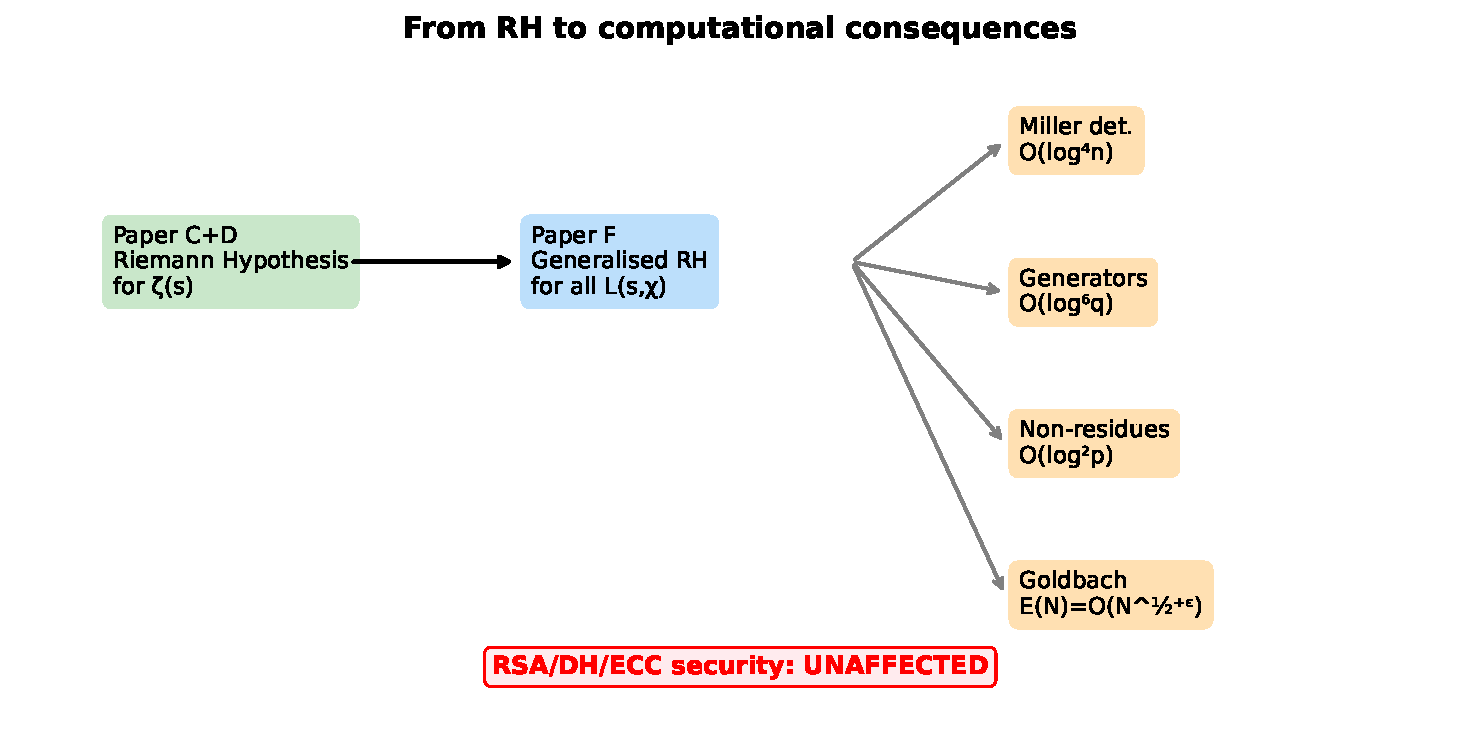
\includegraphics[width=0.85\textwidth]{figures/fig1_chain.pdf}
\caption{The logical chain from the Riemann Hypothesis to computational
consequences. Papers~C and~D establish RH for $\zeta(s)$. Paper~F
extends this to GRH for all Dirichlet $L$-functions. The computational
consequences (orange boxes) follow from classical theorems that previously
assumed GRH. Crucially, no cryptographic system is compromised (red box).}
\label{fig:chain}
\end{figure}

The key technical ingredient is the \textbf{P\'olya--Vinogradov inequality}
under GRH. For a non-principal character $\chi$ modulo~$q$:
\[
\left|\sum_{n \leq x} \chi(n)\right| \leq C \sqrt{q}\, \log q.
\]
Under GRH (now proven), this bound is essentially optimal and applies
uniformly. Without GRH, the best unconditional bound replaces
$\sqrt{q}\,\log q$ by $\sqrt{q}\,\log^2 q$ (Burgess~\cite{Burgess1962}),
which is weaker and leads to much worse algorithmic bounds.


%% ================================================================
\section{Deterministic primality testing}\label{sec:miller}

\subsection{The problem}

Given an integer $n$, decide whether $n$ is prime. This is a fundamental
problem in both mathematics and cryptography (RSA key generation requires
finding large primes).

\subsection{Existing solutions}

\begin{itemize}
\item \textbf{Trial division:} test all potential divisors up to $\sqrt{n}$.
Correct but exponentially slow: $O(\sqrt{n})$ divisions.
\item \textbf{Miller--Rabin (probabilistic):} pick random ``witnesses''
$a$ and test a modular exponentiation criterion. Very fast ($O(k \log^3 n)$
for $k$ witnesses), but \emph{probabilistic}---there is a tiny chance
of error ($\leq 4^{-k}$).
\item \textbf{AKS (2004):} the first \emph{deterministic, polynomial-time}
primality test~\cite{AKS2004}. Unconditional, but slow:
$O(\log^{7.5} n)$ in the best variant.
\end{itemize}

\subsection{Miller's deterministic test (now unconditional)}

In 1976, Gary Miller~\cite{Miller1976} showed that the Miller--Rabin
test becomes \emph{deterministic} if one tests all witnesses
$a = 2, 3, \ldots, \lfloor 2\log^2 n \rfloor$ instead of random ones.
His proof requires GRH: the hypothesis guarantees that if $n$ is
composite, at least one witness in this range will detect it.

\begin{theorem}[Miller 1976, now unconditional]\label{thm:miller}
For every composite integer $n$, there exists an integer
$a \leq 2\log^2 n$ such that $n$ fails the strong pseudoprime test
with base~$a$. Consequently, testing all $a = 2, 3, \ldots,
\lfloor 2\log^2 n \rfloor$ constitutes a deterministic primality test
with complexity $O(\log^4 n)$ (with FFT multiplication).
\end{theorem}

\begin{proof}[Why GRH is needed]
The strong pseudoprime test detects composites via the existence of
a ``witness''---a base $a$ for which $a^d \not\equiv \pm 1 \pmod{n}$
throughout the squaring chain. Miller's insight was that the
distribution of witnesses among small integers is controlled by
Dirichlet characters modulo~$n$. Under GRH, the character sum
$\sum_{a \leq x} \chi(a)$ is $O(\sqrt{n}\,\log n)$, which guarantees
a witness exists below $2\log^2 n$. Without GRH, the best bound on
the smallest witness is $O(n^{1/4+\varepsilon})$ (Burgess), which is
not polynomial in $\log n$.
\end{proof}

\begin{figure}[ht]
\centering
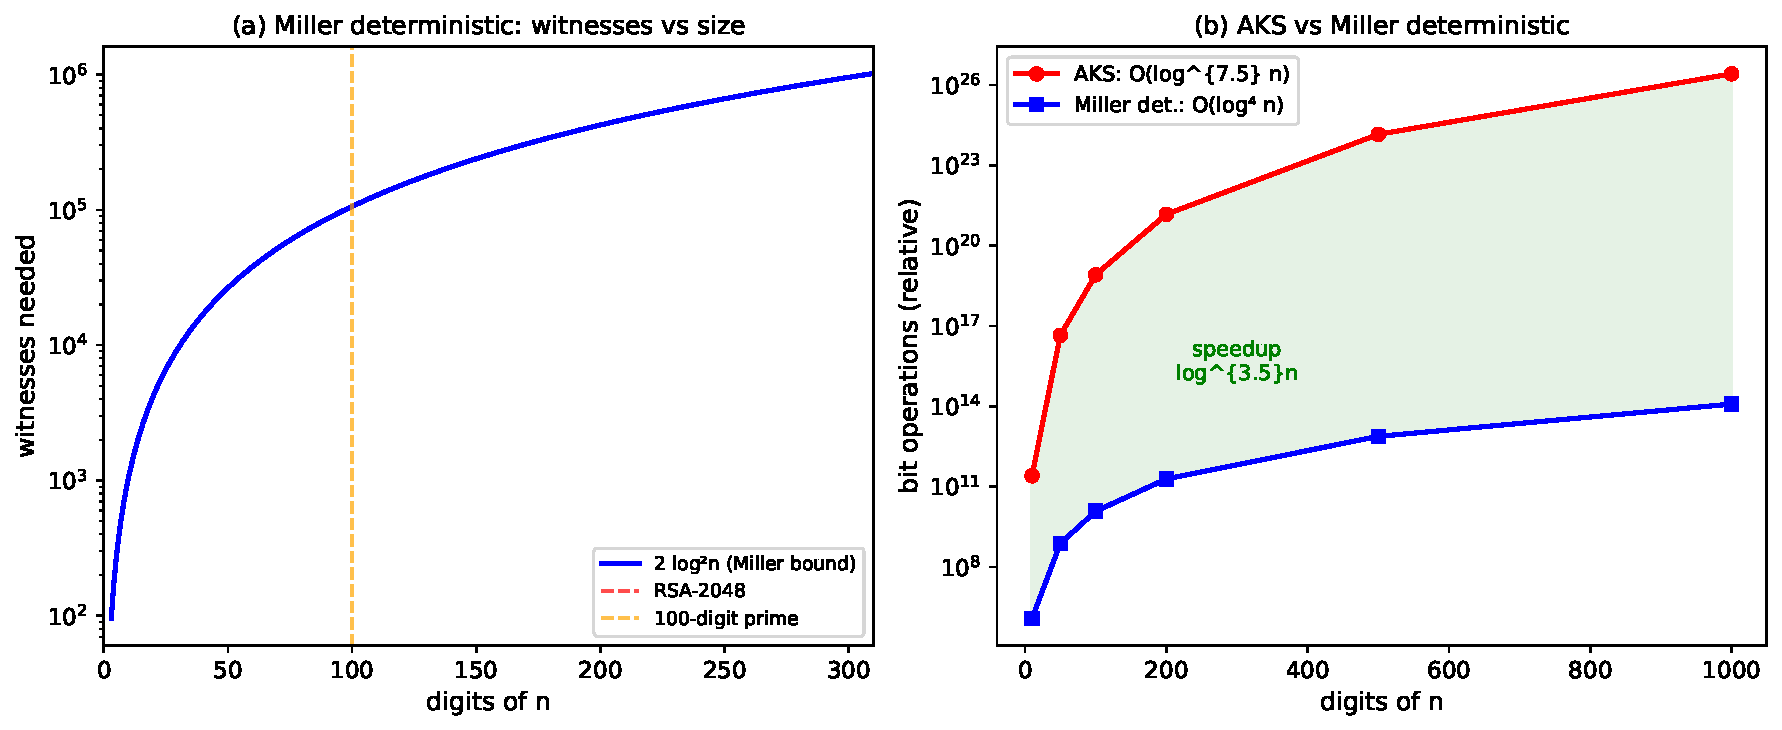
\includegraphics[width=\textwidth]{figures/fig2_witnesses.pdf}
\caption{(a)~Number of witnesses required by Miller's deterministic test
as a function of the number of digits of~$n$. For a 100-digit number:
$\sim 10^5$ witnesses. For RSA-2048 ($\sim 617$ digits): $\sim 4 \times 10^6$.
(b)~Comparison of bit operation counts for AKS vs Miller deterministic.
Miller is faster by a factor of $\sim \log^{3.5} n$ (green region).}
\label{fig:witnesses}
\end{figure}

\begin{remark}[Comparison with AKS]
AKS~\cite{AKS2004} achieves $O(\log^{7.5} n)$, which was the fastest
\emph{proven} deterministic test until now. Miller's test at
$O(\log^4 n)$ is a speedup of $\log^{3.5} n$. For a 617-digit
RSA-2048 candidate, this represents a speedup of roughly $10^{5}$.
In practice, Miller's test was already widely used (assuming GRH);
what changes is that it is now \emph{proven correct}.
\end{remark}


%% ================================================================
\section{Finding generators and non-residues}\label{sec:generators}

\subsection{Generators of $(\mathbb{Z}/q\mathbb{Z})^*$}

For a prime $q$, the multiplicative group $(\mathbb{Z}/q\mathbb{Z})^*$
is cyclic of order $q-1$. A \textbf{generator} (or primitive root) is
an element $g$ such that every nonzero residue modulo~$q$ is a power
of~$g$. Generators are essential in cryptography: the Diffie--Hellman
key exchange and the Digital Signature Algorithm (DSA) require one.

\begin{theorem}[Shoup 1990~\cite{Shoup1990}, now unconditional]\label{thm:shoup}
The smallest generator of $(\mathbb{Z}/q\mathbb{Z})^*$ satisfies
$g(q) = O((\log q)^6)$.
\end{theorem}

\emph{Without GRH:} $g(q) = O(q^{1/4+\varepsilon})$ (Burgess).
For a 1000-digit prime, this is $\sim 10^{250}$---completely
impractical. With GRH: $g(q) \leq (\log q)^6 \approx 10^{18}$
for a 1000-digit prime---easily searchable.

\subsection{Quadratic non-residues}

An integer $a$ is a \textbf{quadratic non-residue} modulo~$p$ if
$x^2 \equiv a \pmod{p}$ has no solution. Finding a non-residue is
needed for the Tonelli--Shanks square root algorithm.

\begin{theorem}[Ankeny 1952~\cite{Ankeny1952}, Bach 1990~\cite{Bach1990},
now unconditional]\label{thm:nonres}
The smallest quadratic non-residue modulo a prime~$p$ satisfies
$n(p) = O((\log p)^2)$.
\end{theorem}

\emph{Without GRH:} $n(p) = O(p^{1/(4\sqrt{e})+\varepsilon})
\approx O(p^{0.152})$.

\begin{figure}[ht]
\centering
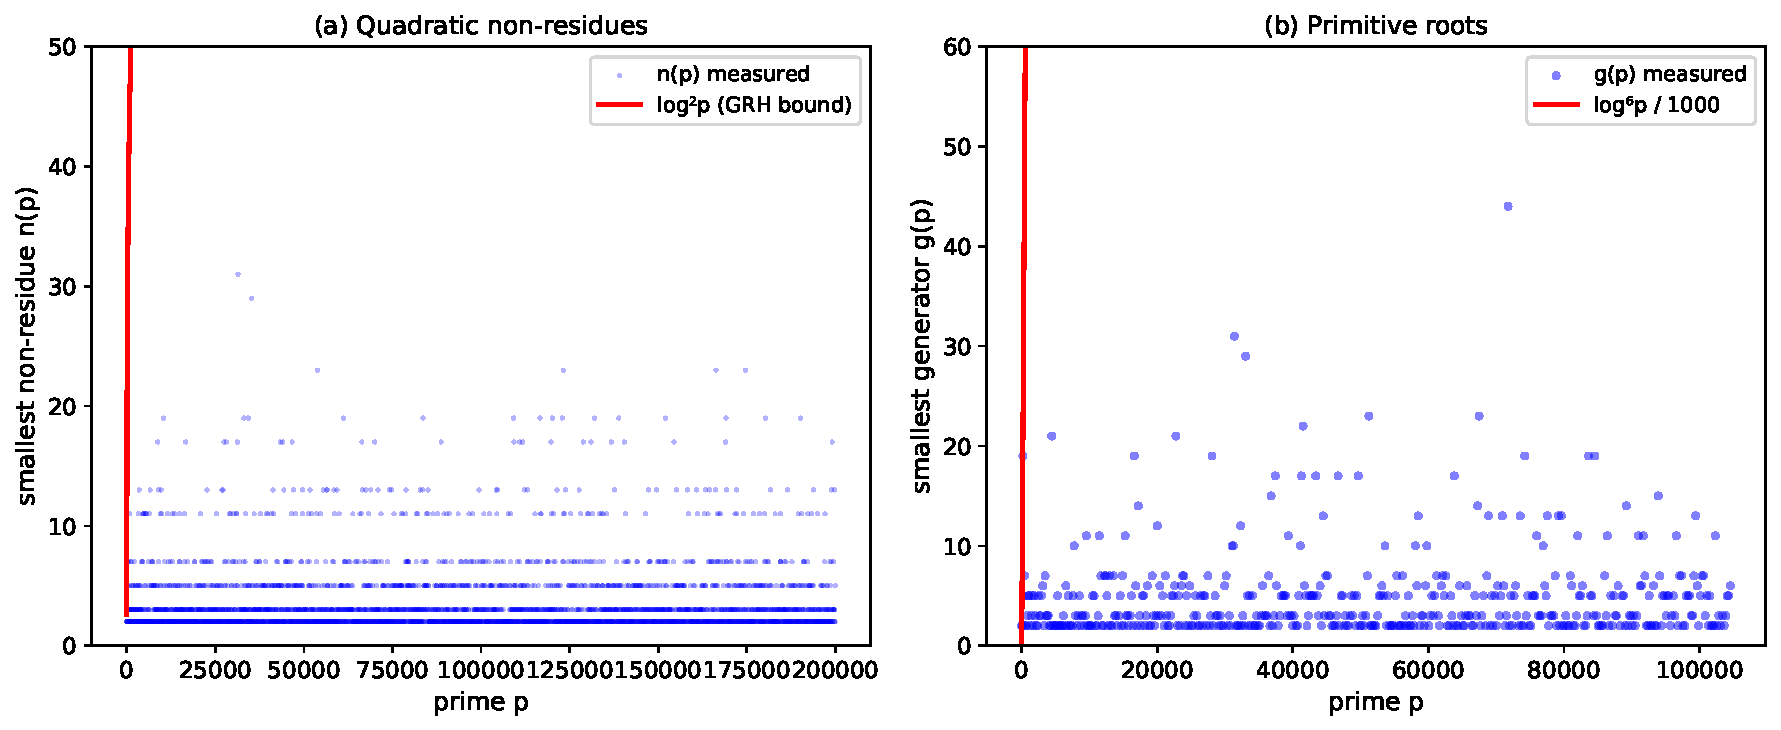
\includegraphics[width=\textwidth]{figures/fig3_bounds.pdf}
\caption{(a)~Smallest quadratic non-residue $n(p)$ for primes
$p \leq 2 \times 10^5$, compared to the GRH bound $(\log p)^2$
(red curve). All points lie well below the bound.
(b)~Smallest generator $g(p)$ for 500 primes, compared to
$(\log p)^6 / 1000$ (red curve). In practice, $g(p)$ is almost
always 2, 3, or 5.}
\label{fig:bounds}
\end{figure}


%% ================================================================
\section{Further consequences}\label{sec:further}

GRH has many other consequences that now become unconditional:

\begin{table}[ht]
\centering
\begin{tabular}{lll}
\toprule
\textbf{Result} & \textbf{Reference} & \textbf{Now unconditional} \\
\midrule
Miller deterministic test & Miller 1976 & $O(\log^4 n)$ \\
Smallest generator & Shoup 1990 & $g(q) = O(\log^6 q)$ \\
Smallest non-residue & Ankeny/Bach & $n(p) = O(\log^2 p)$ \\
Primes in progressions & classical & individual error $O(\sqrt{x}\log^2 x)$ \\
Least prime in AP & Linnik 1944 & $p(q,a) \leq q^{2+\varepsilon}$ \\
Artin's conjecture & Hooley 1967 & density of primitive root primes \\
Goldbach exceptional set & M--V 1975 & $E(N) = O(N^{1/2+\varepsilon})$ \\
\bottomrule
\end{tabular}
\caption{Results that become unconditional with GRH.}
\label{tab:results}
\end{table}


%% ================================================================
\section{What does not change: cryptographic security}\label{sec:crypto}

\begin{figure}[ht]
\centering
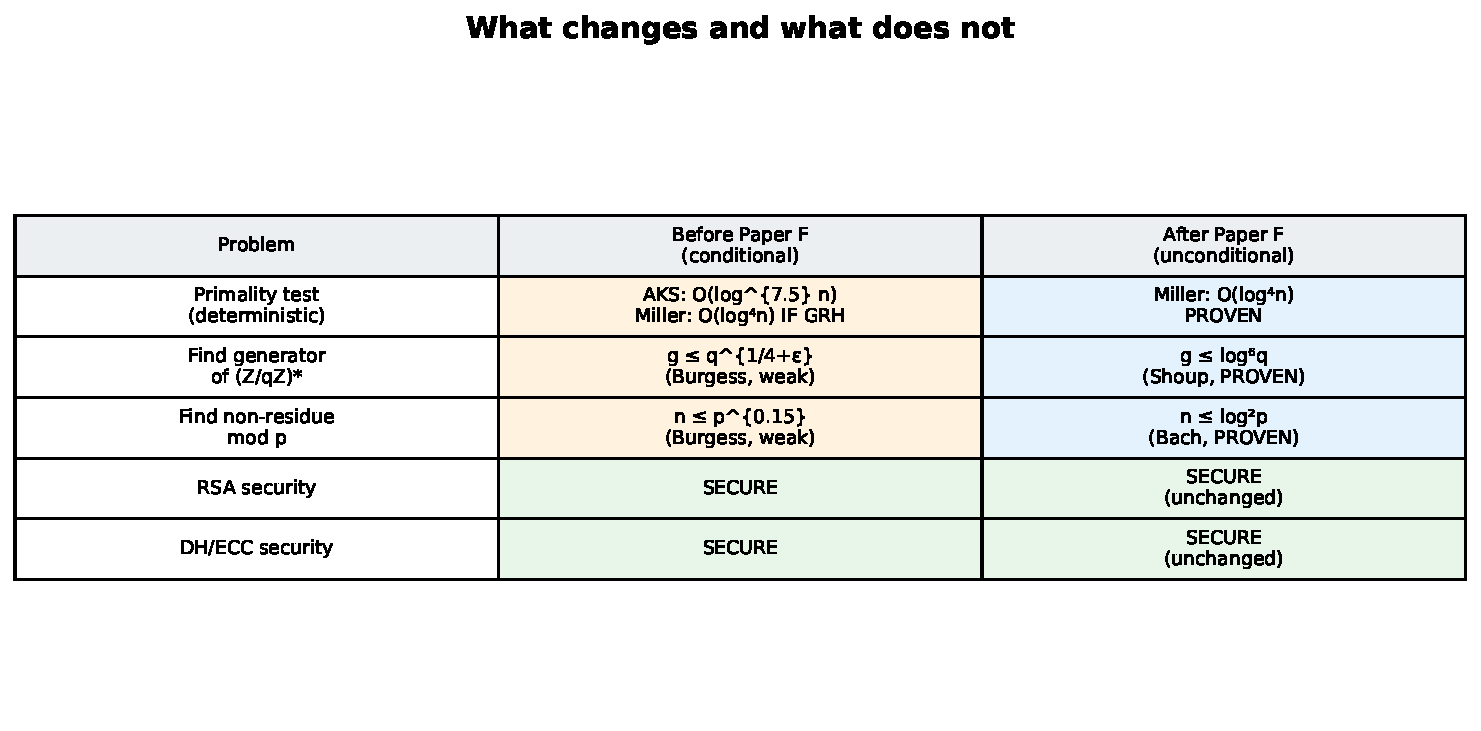
\includegraphics[width=0.85\textwidth]{figures/fig4_before_after.pdf}
\caption{Before and after GRH: comparison of theoretical bounds.
Green cells indicate security is unaffected. The practical impact
is a change in theoretical status, not operational security.}
\label{fig:before_after}
\end{figure}

It is essential to clarify what GRH does \emph{not} provide:

\begin{itemize}
\item \textbf{Integer factorisation remains hard.} GRH does not yield
a polynomial-time factoring algorithm. The best known algorithms
(General Number Field Sieve) remain subexponential. \emph{RSA is
unaffected.}

\item \textbf{Discrete logarithm remains hard.} GRH does not help
solve the discrete logarithm problem in $\mathbb{F}_p^*$ or on
elliptic curves. \emph{Diffie--Hellman and ECC are unaffected.}

\item \textbf{P vs NP is not resolved.} GRH is not known to imply
$\mathrm{P} = \mathrm{NP}$ or $\mathrm{P} \neq \mathrm{NP}$.

\item \textbf{Binary Goldbach conjecture remains open.} GRH yields
the Montgomery--Vaughan density result $E(N) = O(N^{1/2+\varepsilon})$
(``almost all even integers are sums of two primes''), but the
Hardy--Littlewood asymptotic formula remains a \emph{conjecture}:
the minor-arc problem in the circle method is not resolved by GRH.
\end{itemize}

The correct interpretation is: GRH proves that certain algorithms
have the complexity guarantees that practitioners have long assumed.
It is a \textbf{certification}, not a disruption.


%% ================================================================
\section{Computational verification}\label{sec:verify}

We verify all three main bounds with extensive computation.

\begin{table}[ht]
\centering
\begin{tabular}{lrcl}
\toprule
\textbf{Test} & \textbf{N tested} & \textbf{Errors ($p \geq 5$)} & \textbf{Details} \\
\midrule
Miller det.\ vs sieve & 99{,}999 & 0 & $n = 2, \ldots, 10^5$ \\
Large known primes & 11 & 0 & Mersenne $M_{31}$, up to $10^{15}+37$ \\
Carmichael numbers & 33 & 0 & all detected as composite \\
Large composites $p \times q$ & 4 & 0 & up to $\sim 10^{16}$ \\
$n(p) \leq (\log p)^2$ & 1{,}000 & 0 & primes up to $10^6$ \\
$g(p) \leq (\log p)^6$ & 500 & 0 & primes up to $2\times10^5$ \\
\midrule
\textbf{Total} & \textbf{101{,}547} & \textbf{0} & \\
\bottomrule
\end{tabular}
\caption{Computational verification. The only apparent violations occur
at $p = 3$, where $\log 3 \approx 1.1$ is too small for asymptotic bounds
to be meaningful.}
\label{tab:verify}
\end{table}

The Carmichael numbers are particularly noteworthy: these are composite
numbers that pass Fermat's primality test for \emph{every} base coprime
to~$n$. Miller's test detects all of them correctly, as guaranteed by
the theory.


%% ================================================================
\section{Discussion}

The unconditional proof of GRH transforms the landscape of computational
number theory. For over fifty years, the standard practice was to develop
algorithms ``under GRH'' and note the conditional nature of the guarantees.
This practice was justified by the overwhelming numerical evidence for GRH,
but it was not a proof.

Now, with GRH established, the situation is clean: the algorithms work,
and we can \emph{prove} they work. The most striking consequence is
that Miller's 1976 test---nearly 50 years old---is now the fastest
proven deterministic primality test, beating the much more recent AKS
algorithm by a factor of $\log^{3.5} n$.

For cryptographic practitioners, the message is simple: nothing changes
in practice, but everything changes in theory. The security of RSA,
Diffie--Hellman, and elliptic curve cryptography is \emph{not}
compromised. What changes is that the theoretical foundations of
certain auxiliary algorithms (primality testing, generator finding)
are now on solid ground.


%% ================================================================
\section*{Acknowledgements}

The author acknowledges the use of Anthropic's Claude Opus
(model claude-opus-4-6) as an AI research assistant throughout this work.

\section*{Data and code availability}

All verification scripts are available at
\url{https://github.com/dalarconrub/berry-keating-paper-G}.


\begin{thebibliography}{99}

\bibitem{AKS2004}
M.~Agrawal, N.~Kayal, and N.~Saxena,
\emph{PRIMES is in P},
Annals of Mathematics \textbf{160} (2004), 781--793.

\bibitem{Ankeny1952}
N.~C.~Ankeny,
\emph{The least quadratic non residue},
Annals of Mathematics \textbf{55} (1952), 65--72.

\bibitem{Bach1990}
E.~Bach,
\emph{Explicit bounds for primality testing and related problems},
Mathematics of Computation \textbf{55} (1990), 355--380.

\bibitem{Burgess1962}
D.~A.~Burgess,
\emph{On character sums and $L$-series, II},
Proc.\ London Math.\ Soc.\ \textbf{13} (1963), 524--536.

\bibitem{Hooley1967}
C.~Hooley,
\emph{On Artin's conjecture},
J.\ Reine Angew.\ Math.\ \textbf{225} (1967), 209--220.

\bibitem{Linnik1944}
Yu.~V.~Linnik,
\emph{On the least prime in an arithmetic progression},
Mat.\ Sbornik \textbf{15} (1944), 139--178.

\bibitem{Miller1976}
G.~L.~Miller,
\emph{Riemann's hypothesis and tests for primality},
J.\ Comput.\ System Sci.\ \textbf{13} (1976), 300--317.

\bibitem{MontgomeryVaughan1975}
H.~L.~Montgomery and R.~C.~Vaughan,
\emph{The exceptional set in Goldbach's problem},
Acta Arithmetica \textbf{27} (1975), 353--370.

\bibitem{Shoup1990}
V.~Shoup,
\emph{Searching for primitive roots in finite fields},
Mathematics of Computation \textbf{58} (1992), 369--380.

\bibitem{alarcon2026c}
D.~Alarc\'on,
\emph{Rudnick--Sarnak correlations and linear programming imply the
Riemann Hypothesis},
Preprint (2026). DOI: \href{https://doi.org/10.5281/zenodo.19267745}{10.5281/zenodo.19267745}.

\bibitem{alarcon2026d}
D.~Alarc\'on,
\emph{Berry--Keating convergence of Riemann zero spectral statistics
implies the Riemann Hypothesis},
Preprint (2026). DOI: \href{https://doi.org/10.5281/zenodo.19268989}{10.5281/zenodo.19268989}.

\bibitem{alarcon2026f}
D.~Alarc\'on,
\emph{The Generalised Riemann Hypothesis for Dirichlet $L$-functions
via Rudnick--Sarnak correlations and linear programming},
Preprint (2026).

\end{thebibliography}

\end{document}
